\startchapter{Least Squares Localization by Sequential Convex Relaxation}
\label{chapter:scp}

%\textbf{Notes for further development.}
%
%2-step approach:
%
%1) identify outliers to reduce the error-prone data points
%
%2) apply the algorithm  to the redused data set
%
%Projection onto convex sets and projection onto rings \textit{cite GhStr}

%\section{Second Order Cone Programming}

\section{Range-based localization}

Problem:
Given sensor array ${\Ba_i, i = 1, 2, ..., m}$ and noisey range measurements $r_i$ find the true \textit{unknown} location of $\Bx$ as 
\setcounter{abc}{0}
\begin{equation} \label{eq:5.1}
\Min \sum^m_i \left( \|\Bx - \Ba_i\| - r_i \right)^2 
\end{equation}
which can be (equivalently) written as 
\begin{eqnarray} \label{eq:5.2}
\setcounter{abc}{1}
\Min_{\Bx, \Bz}& &\sum^m_i \left( z_i - r_i \right)^2 \\
\setcounter{equation}{2}
\stepcounter{abc}
\mbox{subject to:}& &\|\Bx - \Ba_i\| = z_i, \quad i = 1, 2, ..., m
\end{eqnarray}
The constraint in \ref{eq:5.2} is hard to suffice, therefore we allow a relaxation:
\setcounter{abc}{0}
\begin{eqnarray} \label{eq:5.3}
\setcounter{abc}{1}
\Min_{\Bx, \Bz}& &\sum^m_i \left( z_i - r_i \right)^2 \\
\setcounter{equation}{3}
\stepcounter{abc}
\mbox{subject to:}& &\|\Bx - \Ba_i\| \leq (1+ \gamma)z_i  \\
\setcounter{equation}{3}
\stepcounter{abc}
& &\|\Bx - \Ba_i\| \geq (1 - \gamma)z_i, \quad i = 1, 2, ..., m
\end{eqnarray}
where $\gamma$ is small, typically $0 < \gamma < 0.5$. This would yield an approximate solution to \ref{eq:5.2} and therefore to \ref{eq:5.1}. 
By allowing $\gamma$ to sequentially/monotonically decrease from some small $0 < \gamma_0 < 0.5$ to 0 solution of \ref{eq:5.3} will converge to \ref{eq:5.2}.
\textit{Proof} Let $\gamma(k)$ be monotonically decteasing, where $k$ is an iteration count and $0 < \gamma_0 < 0.5$. Then 
$\lim_{\gamma \rightarrow 0} (1 + \gamma)z_i = z_i$ and $\lim_{\gamma \rightarrow 0} (1 - \gamma)z_i = z_i$. Therefore as $\gamma$ approaches 0, the feasible region of the problem in \ref{eq:5.3} will become equivalent to that in \ref{eq:5.2}.
As iterations proceed, the objective in \ref{eq:5.3} will not be monotonically decreasing but it will converge to the critical point.

Problem in \ref{eq:5.3} is nonconvex due to nonconvexity of one of its inequality constraint. The constraint in \ref{eq:5.3}b $\|\Bx - \Ba_i\| \leq (1+ \gamma)z_i$ is convex, the constraint in \ref{eq:5.3}c is not, because
\begin{equation}
\nonumber
\|\Bx - \Ba_i\| \geq (1 - \gamma)z_i \Longleftrightarrow \underbrace{-\|\Bx - \Ba_i\|}_{nonconvex} \leq -(1 - \gamma)z_i
\end{equation}
From convexity of the norm $\|\Bx - \Ba_i\|$ it follows that for some \textit{known} $\Bx_k$
\begin{equation}
\nonumber
\|\Bx - \Ba_i\| \geq \|\Bx_k - \Ba_i\| + \partial\|\Bx_k - \Ba_i\|^T(\Bx - \Ba_i)
\end{equation}
Hence the constraint in \ref{eq:5.3}c can be convexified by replacing it with its affine approximation
\begin{equation}
\nonumber
-\|\Bx_k - \Ba_i\| - \partial\|\Bx_k - \Ba_i\|^T(\Bx - \Ba_i) \leq -(1 - \gamma)z_i
\end{equation}
At the $k$th iteration when the iterate $\Bx_k$ is known, the nonconvex problem in \ref{eq:5.3} can be converted to an SOCP problem
\setcounter{abc}{0}
\begin{eqnarray} \label{eq:5.4}
\stepcounter{abc}
\Min_{\Bx, \Bz}& &\sum^m_i \left( z_i - r_i \right)^2 \\
\setcounter{equation}{4}
\stepcounter{abc}
\mbox{subject to:}& &\|\Bx - \Ba_i\|  \leq  (1+ \gamma)z_i  
\end{eqnarray}
\begin{equation}
\setcounter{equation}{4}
\stepcounter{abc}
\qquad \qquad \qquad  -\|\Bx_k - \Ba_i\| - \partial\|\Bx_k -\Ba_i\|^T(\Bx - \Ba_i)  \leq  -(1 - \gamma)z_i, \quad i = 1, 2, ..., m
\end{equation}
\setcounter{abc}{0}
The relaxation parameter $\gamma$ controls the size of the convex hull that defines a feasibility region of the problem \ref{eq:5.4}.
$\gamma$ needs to be monotonically decreasing with increase of the iteration count. Start with some $0 < \gamma_0 < 0.5$, typically $\gamma_0 = 0.3$ or 0.2 is good. After $k$th iteration update $\gamma_{k+1}$ linearly as
\begin{equation}
\nonumber
\gamma_{k+1} = \gamma_0 - k\frac{\gamma_0}{K_{max} - 1}
\end{equation}
or quadratically as
\begin{equation}
\nonumber
\gamma_{k+1} = \gamma_0\frac{(K_{max} - 1 - k)^2}{(K_{max} - 1)^2}
\end{equation}


%\startchapter{SOCP}
%\newpage

\section{Range-Difference Localization}

\subsection{Problem Formulation}


In this section we focus on the problem of range-difference based localization given the time-difference of arrival information. TDOA localization, also known as multilateration, or hyperbolic positioning, is a method where the position of the mobile unit (signal source) can be determined using the differences in the TOAs from different base stations. By using this method the clock biases between the mobile units and base stations are automatically removed, since only the pairwise differences between the TOAs from base stations are  considered \cite{LocAlg}.  A hyperbola is the basis for solving multilateration problems. In particular, the set of possible positions of a mobile unit that has a range difference of $d_i$ from two given base stations $BS_i$ and $BS_0$, placed at $\Ba_i$ and $\Ba_0$ respectively, is a hyperbola with vertex separation of $d_i$ and focii located at $\Ba_i$ and $\Ba_0$. $BS_0$ is placed at the origin of the coordinate system, i.e. $\Ba_0 = \symb{0}_n$, and used as a reference station. Consider now a third base station $BS_j$ at a third location. This would provide one extra independent TDOA measurement between $BS_j$ and $BS_0$ and the source is located on the curve determined by the two intersecting hyperboloids. Figure \ref{fig:tdoa} illustrates an example of the range-difference localization based on TDOA measurements.

\begin{figure}[h] 
\centering
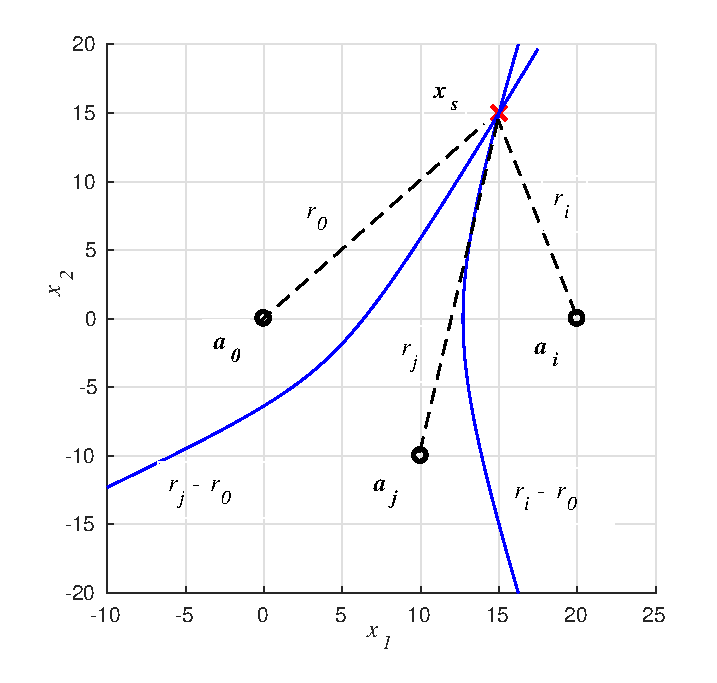
\includegraphics{figures/socp_rd/TDOA_example}
\caption{Range-difference localization.  At least three base stations are required for the planar localization. The red cross indicates the location of the signal source. Sensors are placed at $\protect\Ba_j = (10, -10)^T$, and  $\protect\Ba_0$ is the reference sensor. The time (range) differences $r_j - r_0$ and $r_i - r_0$ form two hyperboloids with focii located at $\protect\Ba_i, \protect\Ba_j$ and $\protect\Ba_0$. Note that the hyperboloids are actually double sheeted, but for visual clarity only the halves which are part of the solution are shown. The intersection of these hyperboloids is the estimated position.
The figure depicts the locus of possible source locations as one half of a two-sheeted hyperboloids.}
\label{fig:tdoa}
\end{figure}
 
%An example of location estimation using TDOA is shown in Figure \ref{fig:hyperbola}. Consider an instance of the source localization problem on the plane $n = 2$ with the reference sensor $\Ba_0$ placed at the origin and five sensors $m = 5$ located at 
%\begin{equation}
%\nonumber
%\Ba_1 = \begin{bmatrix}
%-5 \\ -13
%\end{bmatrix}, \
%\Ba_2 = \begin{bmatrix}
%-12 \\ 1
%\end{bmatrix},  \
%\Ba_3 = \begin{bmatrix}
%-1 \\ -5
%\end{bmatrix}, \
%\Ba_4 = \begin{bmatrix}
%-9 \\ -12
%\end{bmatrix}, \
%\Ba_5 = \begin{bmatrix}
%-3 \\ -12
%\end{bmatrix}
%\\
%\end{equation}
%
%The source emitting the signal was located at $\Bx_s = (-5,11)^T$. Figure \ref{fig:hyperbola} depicts the locus of possible source locations as one half of a two-sheeted hyperboloids.

%\begin{figure} 
%\centering
%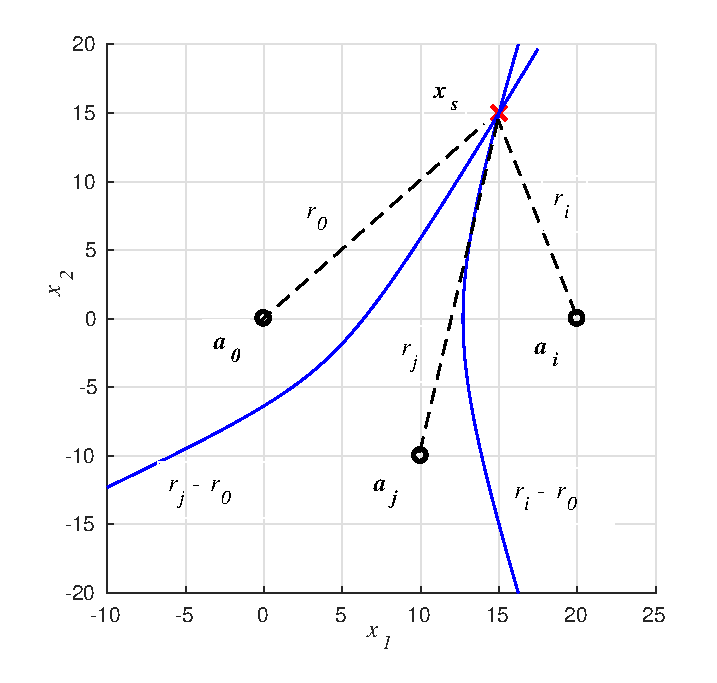
\includegraphics{figures/socp_rd/TDOA_example}
%\caption{Algorithm and contours of the R-LS objective function over the region $\protect\Re = \protect\lbrace \protect\Bx:-15\protect\leq x_1 \protect\leq 15, -25\protect\leq x_2 \protect\leq 15 \protect\rbrace$. The red cross indicates the location of the signal source. Sensors are located at $(-5, -13)^T$, $(-12, 1)^T$, $(-1, -5)^T$, $(-9, -12)^T$ and  $(-3, -12)^T$. Hyperbolas denote possible source locations given the pairwise range-difference readings. Large circles denote possible source locations given the noisy range reading at a particular sensor.}
%\label{fig:hyperbola}
%\end{figure}
 
%Given two base station locations $BS_i$ and $BS_0$, placed at $\Ba_i$ and $\Ba_0$ respectively, with $BS_0$ placed at the origin of the coordinate system, i.e. $\Ba_0 = \symb{0}_n$, and used as a reference station, and a known TDOA, the locus of possible source locations is one half of a two-sheeted hyperboloid. Consider now a third base station $BS_j$ at a third location. This would provide one extra independed TDOA measurement and the source is located on the curve determined by the two intersecting hyperboloids.

%Each TDOA measurement constrains the location of the signal source to be on a hyperboloid with a constant range-difference between the two reference points.

%\textit{Matlab} Using the arrival times, the time differences of arrival between each pair of eNodeBs is calculated using hPositioningTDOA.m. The particular time difference of arrival between a pair of eNodeBs can result from the UE being located at any position where two circles, each centered on an eNodeB, intersect. The two circles have radii which differ by the distance covered at the speed of light in the given time difference. The complete set of possible UE positions across all possible radii for one circle (with the other circle maintaining a radius appropriate to the time difference as already described) forms a hyperbola. The "hyperbolas of constant delay difference" for all the different pairs of eNodeBs are plotted relative to the known eNodeB positions and intersect at the position of the UE.
%A hyperbola is the basis for solving multilateration problems, the task of locating a point from the differences in its distances to given points — or, equivalently, the difference in arrival times of synchronized signals between the point and the given points. Such problems are important in navigation, particularly on water; a ship can locate its position from the difference in arrival times of signals from a LORAN or GPS transmitters. Conversely, a homing beacon or any transmitter can be located by comparing the arrival times of its signals at two separate receiving stations; such techniques may be used to track objects and people. In particular, the set of possible positions of a point that has a distance difference of 2a from two given points is a hyperbola of vertex separation 2a whose foci are the two given points.

%\textit{Wiki} If a pulse is emitted from a platform, it will generally arrive at slightly different times at two spatially separated receiver sites, the TDOA being due to the different distances of each receiver from the platform. In fact, for given locations of the two receivers, a whole set of emitter locations would give the same measurement of TDOA. Given two receiver locations and a known TDOA, the locus of possible emitter locations is one half of a two-sheeted hyperboloid.

%\textit{Wiki} In simple terms, with two receivers at known locations, an emitter can be located onto a hyperboloid.[1] Note that the receivers do not need to know the absolute time at which the pulse was transmitted – only the time difference is needed. A fourth receiver is needed for another independed TDOA, this wil give an extra hyperboloid, the intersection of the curve with this hyperboloid gives one or two solutions, the emitter is then located at the one or at the one of the two solutions.

The localization problem discussed in this section involves a given array of $m+1$ sensors placed in the $n = 2$ or 3 dimentional space with coordinates specified by $\{\Ba_1, \Ba_2, . . . , \Ba_m , a_i \in R^n\}$ and  $\Ba_0 = \symb{0}_n$ placed at the origin and used as a refference sensor. The localization problem here is to estimate the location of a radiating source $\Bx$ given the locations of the $m+1$ sensors and noise-contaminated range-difference measurements $\{d_i, i = 1, 2, \ldots, m\}$ where 
\begin{equation} \label{eq:6.1}
d_i = \|\Bx - \Ba_i\| - \|\Bx\| + \varepsilon_i, \mbox{ for } i = 1, 2, \ldots, m
\end{equation}
Therefore, the standard range-difference LS (RD-LS) problem is formulated as
\begin{equation} \label{eq:6.2}
\Min \sum^m_{i=1}\left( \|\Bx - \Ba_i\| - \|\Bx\| - d_i\right)^2
\end{equation}
As described in Sec.2.2 of the thesis, finding the solution to ($\ref{eq:6.2}$) is a non trivial problem and many approaches have been developed to address this problem. In the following we propose a new iterative procedure to tackle the RD-LS problem (\ref{eq:6.2}), with the goal of achieving a more accurate and robust solution. It operates by  solving an SOCP problem at each iteration to find an increment vector  that sequentially moves the initial estimate of the solution towards the minimum.

\subsection{Sequential SCP}

We begin by re-writing the unconstrained problem in (\ref{eq:6.2}) as a constrained problem with second-order cone constraints%can be equivalently written as
\setcounter{abc}{0}
\begin{eqnarray} \label{eq:6.3} %1.7
\stepcounter{abc}
\setcounter{equation}{7}
\Min_{\Bx, y, \Bz} & & \sum^m_{i=1}\left( z_i - y - d_i\right)^2\\
\stepcounter{abc}
\setcounter{equation}{7}
\mbox{subject to:}& &\|\Bx - \Ba_i\| = z_i \\
\stepcounter{abc}
\setcounter{equation}{7}
& &\|\Bx\|  = y, \quad  i = 1, 2, \ldots m
\end{eqnarray}
Let $\tilde{\Bx} = [\Bx^T \ y \ z_1 \ldots z_m]^T$ with $\Bx \in R^n, y \in R, \Bz \in R^m$ be a known strictly feasible point of the problem in (\ref{eq:6.3}). 
%\setcounter{abc}{0}
%\begin{eqnarray} 
%\nonumber
%\Min_{\Bx, y, \Bz} & & \sum^m_{i=1}\left( z_i - y - d_i\right)^2 \\
%\nonumber
%\mbox{subject to:}& &\|\Bx - \Ba_i\| \leq z_i \\
%\nonumber
%& &\|\Bx\|  \leq y, \quad  i = 1, 2, \ldots m
%\end{eqnarray}
Let $\tilde{\Bdelta} = [\Bdelta_x^T \  \delta_y \ \delta_{z_1} \ \ldots \  \delta_{z_m}]^T$, $\Bdelta_x \in R^n, \Bdelta_y \in R, \Bdelta_z \in R^m$ is a small perturbation to it, such that $|\tilde{\Bdelta}| \leq \beta\symb{1_{m+3}}$ and $\beta > 0$ is a small positive constant. We need to find an increment vector $\tilde{\Bdelta} = [\Bdelta_x^T \  \delta_y \ \Bdelta_{z}^T]^T$ such that the next iterate
\setcounter{abc}{0}
\begin{eqnarray} \label{eq:6.4} %1.8
\stepcounter{abc}
\Bx^{k+1} = \Bx^k + \Bdelta_x \\
\stepcounter{abc}
\setcounter{equation}{8}
y^{k+1} = y^k + \delta_y \\
\stepcounter{abc}
\setcounter{equation}{8}
\Bz^{k+1} = \Bz^k + \Bdelta_z
\end{eqnarray}
remains strictly feasible. 
At the $k+1$th iteration with $\tilde{\Bx}^k$ \textit{known} %update $(\Bx^k, y^k, \Bz^k)$ to 
%Substituting \ref{eq:6.4} in \ref{eq:6.3}
 the objective in \ref{eq:6.3} can be written as
 \setcounter{abc}{0}
\begin{eqnarray} \label{eq:6.5} %1.9
F(\hat{\Bx}) & =  & \sum^m_{i = 1} \left(z^k_i + \delta_{z_i} - (y^k + \delta_y) - d_i \right)^2 \\
\nonumber
& = & \sum^m_{i = 1} \left(- \delta_y + \delta_{z_i}  - \tilde{d_i^k} \right)^2
\end{eqnarray}
where 
\begin{equation}
\nonumber
\tilde{d}^k_i =  d_i - y^k - z_i^k
\end{equation}
 are grouped known constant terms.
Substituting \ref{eq:6.4}b in \ref{eq:6.3}b
\begin{equation}
\nonumber
\|\Bx^k + \Bdelta^k_x - \Ba_i\| = z^k_i +\delta_{z_i}, \quad i = 1, 2, \ldots, m
\end{equation}
The constraints can be convexified by squaring both sides of the equality and then re-grouping the terms on the left-hand side as follows
\begin{eqnarray}
\nonumber
\|(\Bx^k  - \Ba_i) + \Bdelta^k_x\|^2 & = & \left(z^k_i +\delta_{z_i}\right)^2 \\
\nonumber
\Leftrightarrow 
\|\Bx^k  - \Ba_i\|^2 + 2\left( \Bx^k  - \Ba_i \right)^T\Bdelta_x + \cancelto{\mbox{\scriptsize{0}}}{\|\Bdelta_x\|^2}  & = & \left(z_i^k\right)^2 + 2z_i^k\delta_{z_i} + \cancelto{\mbox{\scriptsize{0}}}{\Bdelta^2_{z_i}} \\
\nonumber
\Leftrightarrow \|\Bx^k  - \Ba_i\|^2 + 2\left( \Bx^k  - \Ba_i \right)^T\Bdelta_x   & \approx & \left(z_i^k\right)^2 + 2z_i^k\delta_{z_i} \\
\nonumber
\Leftrightarrow \|\Bx^k  - \Ba_i\|^2 + 2\left( \Bx^k  - \Ba_i \right)^T\Bdelta_x   & \approx & \left(z_i^k\right)^2 + 2z_i^k\delta_{z_i} \\
\nonumber
- 2\left( \Bx^k  - \Ba_i \right)^T\Bdelta_x + 2z_i^k\delta_{z_i}  & \approx & \|\Bx^k  - \Ba_i\|^2 - \left(z_i^k\right)^2
\end{eqnarray}
Repeating the similar procedure with the constraint in \ref{eq:6.3}c
\begin{eqnarray}
\nonumber
\|\Bx^k + \Bdelta_x\| & = & y^k + \delta_y \\
\nonumber
\|\Bx^k + \Bdelta_x\|^2 & = & \left(y^k + \delta_y \right)^2 \\
\nonumber
\Leftrightarrow \|\Bx^k\|^2 + 2\Bdelta_x^T\Bx^k + \cancelto{\mbox{\scriptsize{0}}}{\|\Bdelta_x\|^2} & = & \left(y^k\right)^2 + 2y^k\delta_y +  \cancelto{\mbox{\scriptsize{0}}}{\delta_y^2} \\
\nonumber
\Leftrightarrow -2\left(\Bx^k\right)^T\delta_x + 2y^k\delta & \approx & \|\Bx\|^2 - \left(y^k\right)^2
\end{eqnarray}
The problem in \ref{eq:6.3} can now be written in terms of the \textit{known} feasible  iterate $\tilde{\Bx}^k$ and its \textit{unknown} increment  $\tilde{\Bdelta} = [\Bdelta_x^T \  \delta_y \ \Bdelta_{z}^T]^T$ as
\setcounter{abc}{0}
\begin{eqnarray} \label{eq:6.6} %1.10
\stepcounter{abc}
\Min_{\Bdelta_x, \delta_y, \Bdelta_z}& &\sum^m_{i=1}\left( -\delta_y + \delta_{z_i} -\tilde{d_i}^k\right)^2\\
\setcounter{equation}{10}
\stepcounter{abc}
\mbox{subject to:}& &- 2\left( \Bx^k  - \Ba_i \right)^T\Bdelta_x + 2z_i^k\delta_{z_i}  = \|\Bx^k  - \Ba_i\|^2 - \left(z_i^k\right)^2 \\
\setcounter{equation}{10}
\stepcounter{abc}
& &-2\left(\Bx^k\right)^T\delta_x + 2y^k\delta = \|\Bx^k\|^2 - \left(y^k\right)^2 \\
\setcounter{equation}{10}
\stepcounter{abc}
& &|{\tilde{\Bdelta}}|  \leq \beta\symb{1_{m+3}}, \quad  i = 1, 2, \ldots m
\end{eqnarray}
It is obvious to see that the  problem in \ref{eq:6.6} can be written in the following form
\setcounter{abc}{0}
\begin{eqnarray} \label{eq:6.7} %1.11
\stepcounter{abc}
\Min_{{\Bdelta_x, \delta_y, \Bdelta_z}}& &\| -\delta_y\symb{1_m} + \Bdelta_z - \tilde{\Bd_k} \|_2 
\\ 
\setcounter{equation}{11}
\stepcounter{abc}
\mbox{subject to:}& &\BC_k\tilde{\Bdelta}  = \Bp_k \\
\setcounter{equation}{11}
\stepcounter{abc}
 & &|\tilde{\Bdelta}|  \leq \beta \symb{1_{m+3}}
\end{eqnarray}
where
\setcounter{abc}{0}
\begin{equation} \label{eq:6.8} %12
\tilde{\Bd_k} = 
\begin{bmatrix}
d_1 + y^k - z_1^k \\
d_2 + y^k - z_2^k \\
\vdots \\
d_m + y^k - z_m^k \\
\end{bmatrix}, 
\quad \Bp_k = \begin{bmatrix}
\|\Bx^k\|^2 -\left(y^k\right)^2  \\
\|\Bx^k - \Ba_1\|^2 -\left(z_1^k\right)^2 \\
\vdots \\
\|\Bx^k - \Ba_m\|^2 -\left(z_m^k\right)^2 \\
\end{bmatrix}
\end{equation}
\begin{equation}
\nonumber
\BC_k = \begin{bmatrix}
-2\left(\Bx^k\right)^T & 2y^k & 0 & \hdots & 0 \\
-2\left(\Bx^k - \Ba_1\right)^T & 0 & 2z^k_1 & \hdots & 0 \\
\vdots & \vdots & \vdots & \ddots & \vdots \\
-2\left(\Bx^k - \Ba_m\right)^T & 0 & 0 & \hdots & 2z_m^k
\end{bmatrix},
\quad \tilde{\Bdelta} = \begin{bmatrix}
\Bdelta_x \\
\delta_y \\
\Bdelta_z
\end{bmatrix}
\end{equation}
A technical problem making the formulation in (\ref{eq:6.7}) difficult to implement is that it requires a feasible initial point $\Bx^k$. The iterate $\tilde{\Bx}^k$ is known and  strictly feasible  but it is not guaranteed that the $\tilde{\Bx}^{k+1}$ will also be feasible. The problem can be overcome by introducing nonnegative slack variable $s$ into the constraints in \ref{eq:6.7}c to replace their right-hand sides by relaxed upper bounds (as these new bounds themselves are nonnegative variables). To allow non-feasible increments $\tilde{\Bdelta}$, the problem can be overcome by introducing a
nonnegative slack variable $s \geq 0$ \ref{eq:6.8}c to replace their right-hand sides  by a  relaxed upper bound (as this new bound itself is a nonnegative variable). We allow the constraint in $|\tilde{\Bdelta}|  \leq \beta \symb{1_{m+3}}$ be violated so that the  region with lower value of the objective function can be found. 
This leads to a following sequential relaxation step for the problem in \ref{eq:6.3}
\setcounter{abc}{0}
\begin{eqnarray} \label{eq:6.9} %13
\stepcounter{abc}
\Min_{\Bdelta_x, \delta_y, \Bdelta_z, s}& &\| -\delta_y\symb{1_m} + \Bdelta_z - \tilde{\Bd_k} \|_2 + \mu_ks
\\ 
\stepcounter{abc}
\setcounter{equation}{13}
\mbox{subject to:}& &\BC_k\tilde{\Bdelta}  = \Bp_k 
\\
\stepcounter{abc}
\setcounter{equation}{13}
 & &|\tilde{\Bdelta}|  \leq \left(\beta + s\right)\symb{1_{m+3}} 
 \\
\stepcounter{abc}
\setcounter{equation}{13}
& & s \geq 0
\end{eqnarray}
where the weight $\mu_k \geq 0$ increases as iterations proceed until it reaches an upper limit $\mu_{max}$. By using a monotonically increasing $\mu_k$ for the penalty term in \ref{eq:6.9}a, the algorithm reduces the slack variable $s$  very quickly. As a result, new iterates
quickly become feasible as $s$  vanishes. The upper limit $\mu_{max}$ is imposed to avoid numerical difficulties that may occur if $\mu_{k}$ becomes too large and to ensure convergence if a feasible region is not found.


\subsection{The Algorithm}

Based on the analysis above, the localization algorithm for range-difference measurements can be outlined as follows.

%The constraint $\beta$ was imposed on each element of the vector $\tilde{\Bdelta}$ to guarantee that at each iteration is sufficiently small.

%Dropping the constraints in \ref{eq:6.8}f,g allows more variety in choosing the search direction, which increases the likelihood of the algorithm not to get trapped in the local minimimum.

%\phantom{m}
%\framebox{%
%\parbox{5.4in}{
\label{alg:socp_rd}
%\phantom{m}

\noindent \textbf{Algorithm 4. }

%\phantom{m}

1) Input data: Sensor locations $\{\Ba_i, i=1,\ldots,m\}$, range-difference measurements $\{d_i, i=1,\ldots,m\}$, initial point $\Bx_0$, maximum number of iterations $K_{max}$, initial weight $\mu_0$ and upper limit of weight $\mu_{max}$, increment bound $\beta$. %\gamma, \sigma$, 
Set iteration count to $k = 0$. Form

\begin{equation} 
\setcounter{abc}{0}
\nonumber
y_0 = \|\Bx_0\| ,\quad
\Bz_0 = \begin{bmatrix}
\|\Bx_0 - \Ba_1\|^2  \\
\|\Bx_0 - \Ba_2\|^2  \\
\vdots \\
\|\Bx_0 - \Ba_m\|^2  \\
\end{bmatrix}
\end{equation}

%\phantom{m}

2) Form $\tilde{\Bd_k}, \Bp_k$ and $\BC_k $ as 
\begin{equation} 
\setcounter{abc}{0}
\nonumber
\tilde{\Bd_k} = 
\begin{bmatrix}
d_1 + y^k - z_1^k \\
d_2 + y^k - z_2^k \\
\vdots \\
d_m + y^k - z_m^k \\
\end{bmatrix}, 
\quad \Bp_k = \begin{bmatrix}
\|\Bx^k\|^2 -\left(y^k\right)^2  \\
\|\Bx^k - \Ba_1\|^2 -\left(z_1^k\right)^2 \\
\vdots \\
\|\Bx^k - \Ba_m\|^2 -\left(z_m^k\right)^2 \\
\end{bmatrix}
\end{equation}
\begin{equation}
\nonumber
\BC_k = \begin{bmatrix}
-2\left(\Bx^k\right)^T & 2y^k & 0 & \hdots & 0 \\
-2\left(\Bx^k - \Ba_1\right)^T & 0 & 2z^k_1 & \hdots & 0 \\
\vdots & \vdots & \vdots & \ddots & \vdots \\
-2\left(\Bx^k - \Ba_m\right)^T & 0 & 0 & \hdots & 2z_m^k
\end{bmatrix},
\end{equation}

%\phantom{m}
\noindent
an solve
\setcounter{abc}{0}
\begin{eqnarray} 
\nonumber
\Min_{\Bdelta_x, \delta_y, \Bdelta_z, s}& &\| -\delta_y\symb{1_m} + \Bdelta_z - \tilde{\Bd_k} \|_2 + \mu_ks
\\ 
\nonumber
\mbox{subject to:}& &\BC_k\tilde{\Bdelta}  = \Bp_k 
\\
\nonumber
 & &|\tilde{\Bdelta}|  \leq \left(\beta + s\right)\symb{1_{m+3}} 
 \\
\nonumber
& & s \geq 0
\end{eqnarray}
\noindent
Denote the solution as $\tilde{\Bdelta}^k = (\Bdelta_x^*, \delta_y^*, \Bdelta_z^*)$. 

%\phantom{m}


3) Update  $\mu_{k+1} $ = min $(1.5\mu_k, \mu_{max})$, set $k = k+1$. Update $\tilde{\Bx}^{*}$ to
\setcounter{abc}{0}
\begin{eqnarray} 
\nonumber
\Bx^{*} = \Bx^k + \Bdelta_x^* \\
\nonumber
y^{*} = y^k + \delta_y^* \\
\nonumber
\Bz^{*} = \Bz^k + \Bdelta_z^*
\end{eqnarray}

%\phantom{m}


4) If $k = K_{max}$, terminate and output $\Bx^*$ as the solution; otherwise, set $\tilde{\Bx}^{k} = \tilde{\Bx}^{*}$  and repeat from Step 2. 

%\phantom{m}
%}
%}

\subsection{Numerical Results}

For illustration purposes, the proposed algorithm was applied to a network with five sensors, and its performance was evaluated and compared with existing state-of-the-art methods by Monte Carlo simulations with a set-up similar to that of \cite{BeckStLi}. SR-LS solutions were used as performance benchmarks for the PCCP-based LS Algorithm. The system consisted of $5$ sensors $\{\Ba_i, i = 1, 2,\ldots,5\}$ randomly placed in the planar region in $[-15;15]\times[-15;15]$, and a radiating source $\Bx_s$, located randomly in the region $\{\Bx=[x_1;x_2], -10\leq x_1,x_2\leq 10\}$. The coordinates of the source and sensors were generated for each dimension following a uniform distribution. Measurement noise $\{\varepsilon_i, i=1,\ldots,m\}$ was modelled as independent and identically distributed (i.i.d) random variables with zero mean and variance $\sigma^2$, with $\sigma$ being one of four possible levels $\{10^{-3}, 10^{-2}, 10^{-1}, 1\}$.  The range-difference measurements $\{d_i, i=1, 2,\ldots,5\}$ were calculated using (\ref{eq:6.1}). Accuracy of source location estimation was evaluated in terms of average of the squared position error error in the form $\|\Bx^*-\Bx_s\|^2$, where $\Bx_s$ denotes the exact source location and $\Bx^*$ is its estimation obtained by SR-LS and proposed methods, respectively.  
In our simulations parameter $\beta$ was set to () and the number of iterations was set to (). The proposed method was implemented by using  CVX  \cite{cvx} and implementation of SRD-LS followed \cite{BeckStLi}. The proposed algorithm was initialized with ...  